\documentclass[mstat,12pt]{unswthesis}

\usepackage{color}
\usepackage{fancyvrb}
\newcommand{\VerbBar}{|}
\newcommand{\VERB}{\Verb[commandchars=\\\{\}]}
\DefineVerbatimEnvironment{Highlighting}{Verbatim}{commandchars=\\\{\}}
% Add ',fontsize=\small' for more characters per line
\usepackage{framed}
\definecolor{shadecolor}{RGB}{248,248,248}
\newenvironment{Shaded}{\begin{snugshade}}{\end{snugshade}}
\newcommand{\AlertTok}[1]{\textcolor[rgb]{0.94,0.16,0.16}{#1}}
\newcommand{\AnnotationTok}[1]{\textcolor[rgb]{0.56,0.35,0.01}{\textbf{\textit{#1}}}}
\newcommand{\AttributeTok}[1]{\textcolor[rgb]{0.13,0.29,0.53}{#1}}
\newcommand{\BaseNTok}[1]{\textcolor[rgb]{0.00,0.00,0.81}{#1}}
\newcommand{\BuiltInTok}[1]{#1}
\newcommand{\CharTok}[1]{\textcolor[rgb]{0.31,0.60,0.02}{#1}}
\newcommand{\CommentTok}[1]{\textcolor[rgb]{0.56,0.35,0.01}{\textit{#1}}}
\newcommand{\CommentVarTok}[1]{\textcolor[rgb]{0.56,0.35,0.01}{\textbf{\textit{#1}}}}
\newcommand{\ConstantTok}[1]{\textcolor[rgb]{0.56,0.35,0.01}{#1}}
\newcommand{\ControlFlowTok}[1]{\textcolor[rgb]{0.13,0.29,0.53}{\textbf{#1}}}
\newcommand{\DataTypeTok}[1]{\textcolor[rgb]{0.13,0.29,0.53}{#1}}
\newcommand{\DecValTok}[1]{\textcolor[rgb]{0.00,0.00,0.81}{#1}}
\newcommand{\DocumentationTok}[1]{\textcolor[rgb]{0.56,0.35,0.01}{\textbf{\textit{#1}}}}
\newcommand{\ErrorTok}[1]{\textcolor[rgb]{0.64,0.00,0.00}{\textbf{#1}}}
\newcommand{\ExtensionTok}[1]{#1}
\newcommand{\FloatTok}[1]{\textcolor[rgb]{0.00,0.00,0.81}{#1}}
\newcommand{\FunctionTok}[1]{\textcolor[rgb]{0.13,0.29,0.53}{\textbf{#1}}}
\newcommand{\ImportTok}[1]{#1}
\newcommand{\InformationTok}[1]{\textcolor[rgb]{0.56,0.35,0.01}{\textbf{\textit{#1}}}}
\newcommand{\KeywordTok}[1]{\textcolor[rgb]{0.13,0.29,0.53}{\textbf{#1}}}
\newcommand{\NormalTok}[1]{#1}
\newcommand{\OperatorTok}[1]{\textcolor[rgb]{0.81,0.36,0.00}{\textbf{#1}}}
\newcommand{\OtherTok}[1]{\textcolor[rgb]{0.56,0.35,0.01}{#1}}
\newcommand{\PreprocessorTok}[1]{\textcolor[rgb]{0.56,0.35,0.01}{\textit{#1}}}
\newcommand{\RegionMarkerTok}[1]{#1}
\newcommand{\SpecialCharTok}[1]{\textcolor[rgb]{0.81,0.36,0.00}{\textbf{#1}}}
\newcommand{\SpecialStringTok}[1]{\textcolor[rgb]{0.31,0.60,0.02}{#1}}
\newcommand{\StringTok}[1]{\textcolor[rgb]{0.31,0.60,0.02}{#1}}
\newcommand{\VariableTok}[1]{\textcolor[rgb]{0.00,0.00,0.00}{#1}}
\newcommand{\VerbatimStringTok}[1]{\textcolor[rgb]{0.31,0.60,0.02}{#1}}
\newcommand{\WarningTok}[1]{\textcolor[rgb]{0.56,0.35,0.01}{\textbf{\textit{#1}}}}


%%%%%%%%%%%%%%%%%%%%%%%%%%%%%%%%%%%%%%%%%%%%%%%%%%%%%%%%%%%%%%%%%%
% 
% OK...Now we get to some actual input.  The first part sets up
% the title etc that will appear on the front page
%
%%%%%%%%%%%%%%%%%%%%%%%%%%%%%%%%%%%%%%%%%%%%%%%%%%%%%%%%%%%%%%%%%

\title{Capstone Project by Team 3\\[0.5cm]A Data Science Approach to
Forecast Short-term Electricity Demand in NSW}

\authornameonly{Karim Adham (z5468227), Rishantha Rajakaruna
(z5441528), Rushmila Islam (z5456038) }

\author{\Authornameonly}

\copyrightfalse
\figurespagefalse
\tablespagefalse

%%%%%%%%%%%%%%%%%%%%%%%%%%%%%%%%%%%%%%%%%%%%%%%%%%%%%%%%%%%%%%%%%
%
%  And now the document begins
%  The \beforepreface and \afterpreface commands puts the
%  contents page etc in
%
%%%%%%%%%%%%%%%%%%%%%%%%%%%%%%%%%%%%%%%%%%%%%%%%%%%%%%%%%%%%%%%%%%


%%%%%%%%%%%%%%%%%%%%%%%%%%%%%%%%%%%%%%%%%%%%%%%%%%%%%%%%%%%%%%%%%%%%%%%
%
%  A small sample UNSW Coursework Masters thesis file.
%  Any questions to Ian Doust i.doust@unsw.edu.au and/or Gery Geenens ggeenens@unsw.edu.au
%
%%%%%%%%%%%%%%%%%%%%%%%%%%%%%%%%%%%%%%%%%%%%%%%%%%%%%%%%%%%%%%%%%%%%%%%
%
%  The first part pulls in a UNSW Thesis class file.  This one is
%  slightly nonstandard and has been set up to do a couple of
%  things automatically
%
 
%%%%%%%%%%%%%%%%%
%% Precisely one of the next four lines should be uncommented.
%% Choose the one which matches your degree, uncomment it, and comment out the other two!
%\documentclass[mfin,12pt]{unswthesis}    %%  For Master of Financial Mathematics 
%\documentclass[mmath,12pt]{unswthesis}   %%  For Master of Mathematics
%\documentclass[mstat,12pt]{unswthesis}  %%  For Master of Statistics
%%%%%%%%%%%%%%%%%



\linespread{1}
\usepackage{amsfonts}
\usepackage{amssymb}
\usepackage{amsthm}
\usepackage{latexsym,amsmath}
\usepackage{graphicx}
\usepackage{afterpage}
\usepackage[colorlinks]{hyperref}
 \hypersetup{
     colorlinks=true,
     linkcolor=blue,
     filecolor=blue,
     citecolor= black,      
     urlcolor=cyan,
     }
\usepackage{textcomp}
\usepackage{longtable}
\usepackage{booktabs}
\usepackage{float}

%%%%%%%%%%%%%%%%%%%%%%%%%%%%%%%%%%%%%%%%%%%%%%%%%%%%%%%%%%%%%%%%%
%
%  The following are some simple LaTeX macros to give some
%  commonly used letters in funny fonts. You may need more or less of
%  these
%
\newcommand{\R}{\mathbb{R}}
\newcommand{\Q}{\mathbb{Q}}
\newcommand{\C}{\mathbb{C}}
\newcommand{\N}{\mathbb{N}}
\newcommand{\F}{\mathbb{F}}
\newcommand{\PP}{\mathbb{P}}
\newcommand{\T}{\mathbb{T}}
\newcommand{\Z}{\mathbb{Z}}
\newcommand{\B}{\mathfrak{B}}
\newcommand{\BB}{\mathcal{B}}
\newcommand{\M}{\mathfrak{M}}
\newcommand{\X}{\mathfrak{X}}
\newcommand{\Y}{\mathfrak{Y}}
\newcommand{\CC}{\mathcal{C}}
\newcommand{\E}{\mathbb{E}}
\newcommand{\cP}{\mathcal{P}}
\newcommand{\cS}{\mathcal{S}}
\newcommand{\A}{\mathcal{A}}
\newcommand{\ZZ}{\mathcal{Z}}
%%%%%%%%%%%%%%%%%%%%%%%%%%%%%%%%%%%%%%%%%%%%%%%%%%%%%%%%%%%%%%%%%%%%%
%
% The following are much more esoteric commands that I have left in
% so that this file still processes. Use or delete as you see fit
%
\newcommand{\bv}[1]{\mbox{BV($#1$)}}
\newcommand{\comb}[2]{\left(\!\!\!\begin{array}{c}#1\\#2\end{array}\!\!\!\right)
}
\newcommand{\Lat}{{\rm Lat}}
\newcommand{\var}{\mathop{\rm var}}
\newcommand{\Pt}{{\mathcal P}}
\def\tr(#1){{\rm trace}(#1)}
\def\Exp(#1){{\mathbb E}(#1)}
\def\Exps(#1){{\mathbb E}\sparen(#1)}
\newcommand{\floor}[1]{\left\lfloor #1 \right\rfloor}
\newcommand{\ceil}[1]{\left\lceil #1 \right\rceil}
\newcommand{\hatt}[1]{\widehat #1}
\newcommand{\modeq}[3]{#1 \equiv #2 \,(\text{mod}\, #3)}
\newcommand{\rmod}{\,\mathrm{mod}\,}
\newcommand{\p}{\hphantom{+}}
\newcommand{\vect}[1]{\mbox{\boldmath $ #1 $}}
\newcommand{\reff}[2]{\ref{#1}.\ref{#2}}
\newcommand{\psum}[2]{\sum_{#1}^{#2}\!\!\!'\,\,}
\newcommand{\bin}[2]{\left( \begin{array}{@{}c@{}}
				#1 \\ #2
			\end{array}\right)	}
%
%  Macros - some of these are in plain TeX (gasp!)
%
\newcommand{\be}{($\beta$)}
\newcommand{\eqp}{\mathrel{{=}_p}}
\newcommand{\ltp}{\mathrel{{\prec}_p}}
\newcommand{\lep}{\mathrel{{\preceq}_p}}
\def\brack#1{\left \{ #1 \right \}}
\def\bul{$\bullet$\ }
\def\cl{{\rm cl}}
\let\del=\partial
\def\enditem{\par\smallskip\noindent}
\def\implies{\Rightarrow}
\def\inpr#1,#2{\t \hbox{\langle #1 , #2 \rangle} \t}
\def\ip<#1,#2>{\langle #1,#2 \rangle}
\def\lp{\ell^p}
\def\maxb#1{\max \brack{#1}}
\def\minb#1{\min \brack{#1}}
\def\mod#1{\left \vert #1 \right \vert}
\def\norm#1{\left \Vert #1 \right \Vert}
\def\paren(#1){\left( #1 \right)}
\def\qed{\hfill \hbox{$\Box$} \smallskip}
\def\sbrack#1{\Bigl \{ #1 \Bigr \} }
\def\ssbrack#1{ \{ #1 \} }
\def\smod#1{\Bigl \vert #1 \Bigr \vert}
\def\smmod#1{\bigl \vert #1 \bigr \vert}
\def\ssmod#1{\vert #1 \vert}
\def\sspmod#1{\vert\, #1 \, \vert}
\def\snorm#1{\Bigl \Vert #1 \Bigr \Vert}
\def\ssnorm#1{\Vert #1 \Vert}
\def\sparen(#1){\Bigl ( #1 \Bigr )}

\newcommand\blankpage{%
    \null
    \thispagestyle{empty}%
    \addtocounter{page}{-1}%
    \newpage}

%%%%%%%%%%%%%%%%%%%%%%%%%%%%%%%
%
% These environments allow you to get nice numbered headings
%  for your Theorems, Definitions etc.  
%
%  Environments
%
%%%%%%%%%%%%%%%%%%%%%%%%%%%%%%%

\newtheorem{theorem}{Theorem}[section]
\newtheorem{lemma}[theorem]{Lemma}
\newtheorem{proposition}[theorem]{Proposition}
\newtheorem{corollary}[theorem]{Corollary}
\newtheorem{conjecture}[theorem]{Conjecture}
\newtheorem{definition}[theorem]{Definition}
\newtheorem{example}[theorem]{Example}
\newtheorem{remark}[theorem]{Remark}
\newtheorem{question}[theorem]{Question}
\newtheorem{notation}[theorem]{Notation}
\numberwithin{equation}{section}

%%%%%%%%%%%%%%%%%%%%%%%%%%%%%%%%%%%%%%%%%%%%%%%%%%%%%%%%%%%%%%%%%%
%
%  If you've got some funny special words that LaTeX might not
% hyphenate properly, you can give it a helping hand:
%

\hyphenation{Mar-cin-kie-wicz Rade-macher}


\newlength{\cslhangindent}
\setlength{\cslhangindent}{1.5em}
\newlength{\csllabelwidth}
\setlength{\csllabelwidth}{3em}
\newenvironment{CSLReferences}[2] % #1 hanging-ident, #2 entry spacing
 {% don't indent paragraphs
  \setlength{\parindent}{0pt}
  % turn on hanging indent if param 1 is 1
  \ifodd #1 \everypar{\setlength{\hangindent}{\cslhangindent}}\ignorespaces\fi
  % set entry spacing
  \ifnum #2 > 0
  \setlength{\parskip}{#2\baselineskip}
  \fi
 }%
 {}
\usepackage{calc} % for \widthof, \maxof
\newcommand{\CSLBlock}[1]{#1\hfill\break}
\newcommand{\CSLLeftMargin}[1]{\parbox[t]{\maxof{\widthof{#1}}{\csllabelwidth}}{#1}}
\newcommand{\CSLRightInline}[1]{\parbox[t]{\linewidth}{#1}}
\newcommand{\CSLIndent}[1]{\hspace{\cslhangindent}#1}

\bibliographystyle{elsarticle-num}




\begin{document}

\beforepreface

%\afterpage{\blankpage}

% plagiarism

\prefacesection{Plagiarism statement}

\vskip 2pc \noindent I declare that this thesis is my
own work, except where acknowledged, and has not been submitted for
academic credit elsewhere. 

\vskip 2pc  \noindent I acknowledge that the assessor of this
thesis may, for the purpose of assessing it:
\begin{itemize}
\item Reproduce it and provide a copy to another member of the University; and/or,
\item Communicate a copy of it to a plagiarism checking service (which may then retain a copy of it on its database for the purpose of future plagiarism checking).
\end{itemize}

\vskip 2pc \noindent I certify that I have read and understood the University Rules in
respect of Student Academic Misconduct, and am aware of any potential plagiarism penalties which may 
apply.\vspace{24pt}

\vskip 2pc \noindent By signing 
this declaration I am
agreeing to the statements and conditions above.
\vskip 2pc \noindent
Signed: \rule{7cm}{0.25pt} \hfill Date: \rule{4cm}{0.25pt} \\[1cm]
Signed: \rule{7cm}{0.25pt} \hfill Date: \rule{4cm}{0.25pt} \\[1cm]
Signed: \rule{7cm}{0.25pt} \hfill Date: \rule{4cm}{0.25pt} \\[1cm]
\vskip 1pc

%\afterpage{\blankpage}

% Acknowledgements are optional


\prefacesection{Acknowledgements}

{\bigskip}TBW\ldots{}\\[1cm] 

{\bigskip\bigskip\bigskip\noindent} 02/10/2024.

%\afterpage{\blankpage}

% Abstract

\prefacesection{Abstract}

TBW \ldots{}

%\afterpage{\blankpage}


\afterpreface





%%%%%%%%%%%%%%%%%%%%%%%%%%%%%%%%%%%%%%%%%%%%%%%%%%%%%%%%%%%%%%%%%%
%
% Now we can start on the first chapter
% Within chapters we have sections, subsections and so forth
%
%%%%%%%%%%%%%%%%%%%%%%%%%%%%%%%%%%%%%%%%%%%%%%%%%%%%%%%%%%%%%%%%%%



%%%%%%%%%%%%%%%%%%%%%%%%%%%%%%%%%%%%%

%\afterpage{\blankpage}


\chapter{Introduction}\label{introduction}

This R Markdown template can be used for the ZZSC9020 course report. You
can incorporate R \cite{R} chunks and Python chunks that will be run on
the fly. You can incorporate \LaTeX commands.

\bigskip

TBW

\chapter{Literature Review}\label{literature-review}

\section{Background}\label{background}

Electricity demand forecasting is crucial for ensuring an efficient,
reliable and cost-effective power operation systems. Accurate forecasts
enable grid operators to balance supply and demand in real-time,
preventing costly overproduction or dangerous shortages that could lead
to blackouts. It also helps to optimize the scheduling of power
generation for different sectors, reducing operational costs and
enhancing system reliability. As renewable energy sources like solar and
wind become more integrated, forecasting plays a vital role in managing
fluctuations in supply. Additionally, in deregulated markets, precise
demand predictions allow energy providers to make informed trading
decisions, ultimately benefiting both suppliers and consumers with more
stable and affordable electricity.

NSW is largely self-sufficient in relation to electricity supply
according to \cite{nswEnergyConsumption2021}, meeting most of its local
demand through state generation. The remaining electricity is purchased
from other states through the National Electricity Market (NEM).
Electricity imports enable NSW to manage its supply at the lowest cost
to consumers. In 2019--20, renewable energy sources accounted for
approximately 19\% of the state's total electricity generation, a
significant increase from just over four times the amount in 2008--09.

According to \cite{nsw_epa_2021_energy_consumption} electricity demand
from the NSW grid is projected to experience a slight decline over the
next five years before rising more. As stated in the ariticle the main
reason for the decline in energy consumption is the lower consumption by
the NSW industrial sector, particularly the manufacturing industry,
since 2012--13. Industrial energy consumption saw a marked decline after
the closure of the Kurnell and Clyde petroleum refineries in October
2014, with few significant changes observed since then. The decrease is
expected to be driven by population growth being balanced by
improvements in the energy efficiency of appliances and machinery. In
addition, the increasing adoption of rooftop solar panels and battery
storage systems is anticipated to further lower residential demand on
the electricity grid. However, beyond the five-year mark, consumption is
forecasted to increase as electric vehicle charging and broader
electrification begin to significantly impact electricity demand.
According to NSW Climate and Energy Action. (n.d.) the share of solar
and wind in NSW's energy mix has more than DOUBLED from 5\% in 2015 to
12\% in 2019. In the Figure \ref{renewable} we can visualize the rapid
growth of electricity generation using renewable sources.

\begin{figure}[H]
\centering
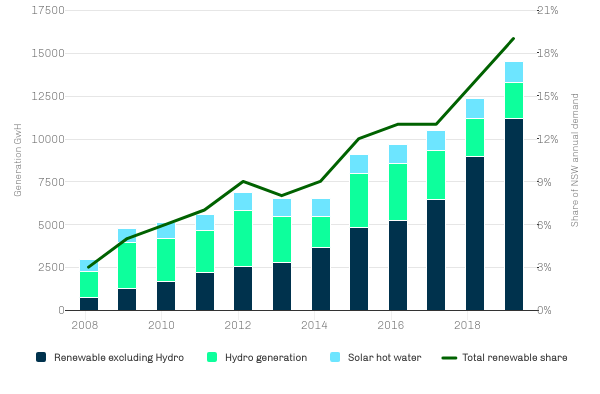
\includegraphics[width=0.95\textwidth,height=10cm]{renewable_fuel_sources_chart.png}
\caption{Renewable fuel sources [Source:
Derived from Department of the Environment and Energy, Australian Energy Statistics, Table O, June 2021]}\label{renewable}
\end{figure}

As stated in \cite{nswEnergyConsumption} the driving factors of
electricity consumption and demand forecasts can be split into two
different types: structural drivers and random drivers. Structural
drivers such as population, economic growth, electricity price,
technology adoption, energy efficiency can be estimated based on past
trends and expert judgement. On the other hand, random drivers, such as
weather, customer behavior etc, which can be modeled as probability
distributions. There are many factors that drive consumers to make
similar choices regarding electricity consumption at the same time for
example during work and school schedules. And the demand is different
during weekdays, public holidays, weekends, due to weather the use of
heating and cooling appliances, and many other societal factors, such as
whether the beach is pleasant, or the occurrence of retail promotions.

Load forecasting is usually concerned with the prediction of hourly,
daily, weekly, and annual values of the system demand and peak demand.
Such forecasts are sometimes categorized as short-term, medium-term and
long-term forecasts, depending on the time horizon. In terms of
forecasting outputs, load forecasts can also be categorized as point
forecasts (i.e., forecasts of the mean or median of the future demand
distribution), and density forecasts (providing estimates of the full
probability distributions of the possible future values of the demand).

\section{Factors Affecting Load
Forecasting}\label{factors-affecting-load-forecasting}

In addition to the basic components of electricity demand forecasting,
several external factors play a significant role in refining predictions
and improving accuracy. Typically, electricity consumption is influenced
by two factors---1) structural like population growth, economic
condition, electricity price, etc; and 2) non-structural or random like
weather condition e.g., air temperature, extreme heat or cold, bushfire,
flood, etc., building type e.g., multi-storey or free-standing house,
and adoption of electric vehicles and contributions of renewable energy
in the power grid, etc.

Temperature is a crucial factor, as it directly influences electricity
consumption patterns. Extreme temperatures, whether very hot or cold,
can lead to higher demand for heating or cooling, respectively.
Forecasts often need to account for temperature variations to predict
demand more accurately, especially during seasonal extremes or unusual
weather patterns.

\begin{figure}[H]
\centering
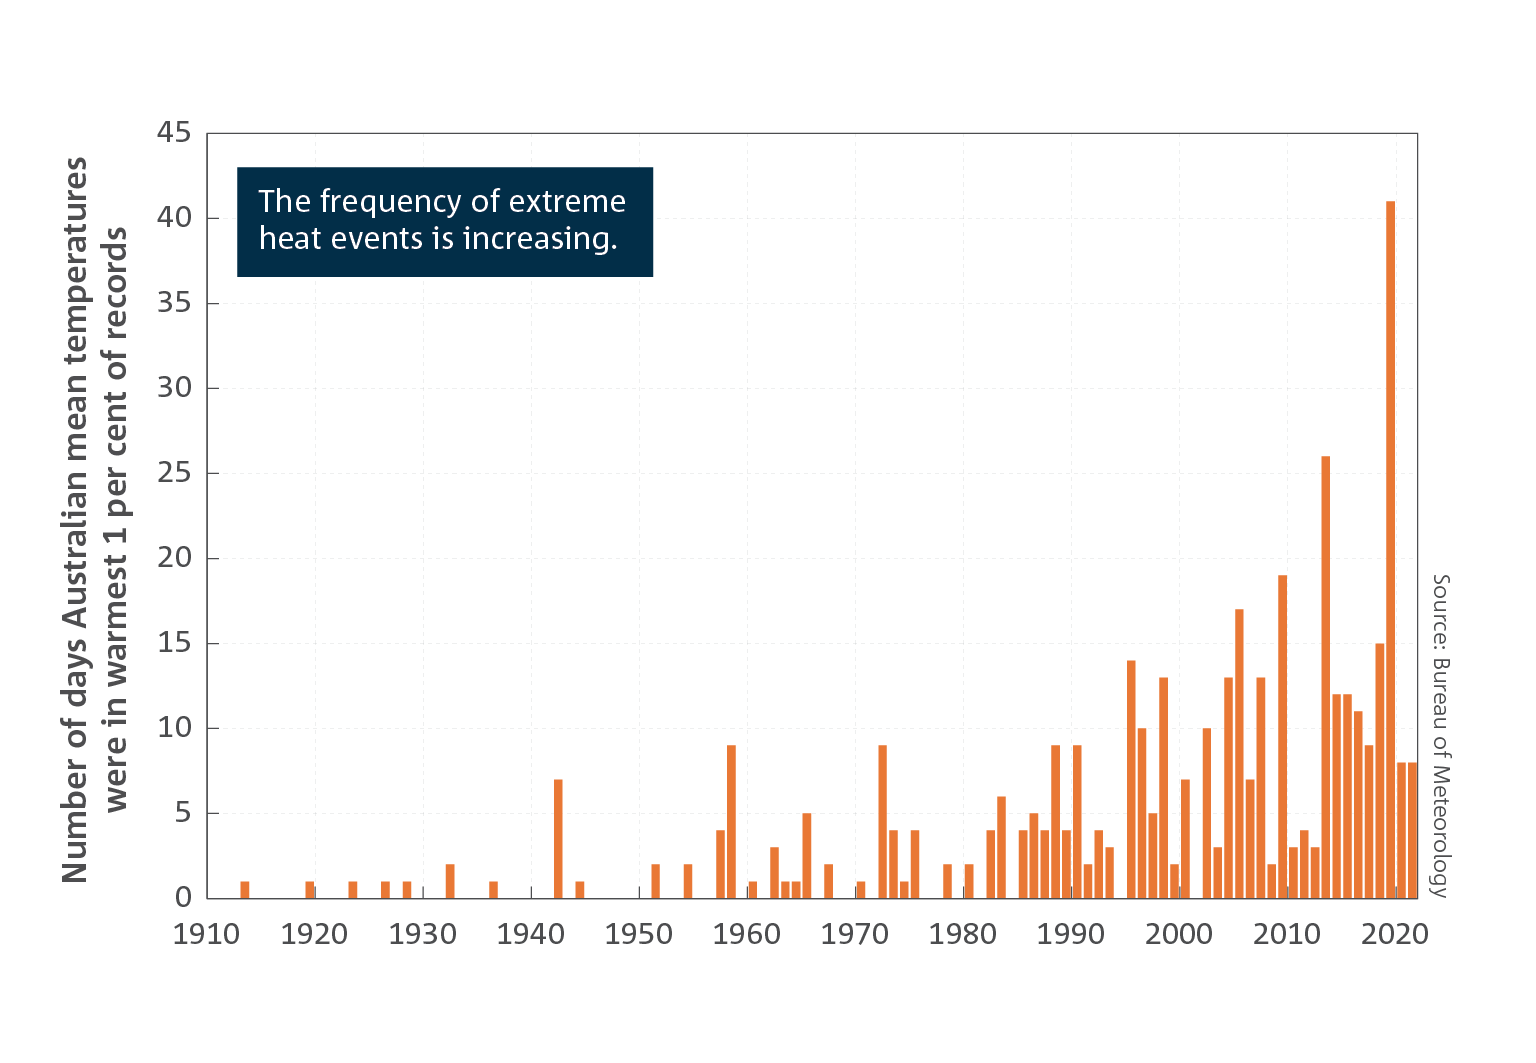
\includegraphics[width=0.95\textwidth, height=10cm]{extreme_temp__au.png}
\caption{A caption1}\label{extreme}
\end{figure}

As the graph in Figure \ref{extreme} shows the temperature in Australia
is rising and forecast show that it will continue to rise. According to
\cite{nswAdaptNSW} the climate of NSW is changing, with 6 of the 10
warmest years on record occurring in the past 10 years. The warmest year
on record for both average temperature and maximum temperature in NSW
was 2019, when average temperature was 1.2°C above the 1990--2009
average. Across NSW, average temperatures will continue to increase
throughout this century. By 2090, average temperature is projected to
rise by around 1.3°C under a low emissions scenario and around 4.0°C
under a high emissions scenario. So temperature is key factor while
determining the electricity demand. The usage of heating in colder
nights and cooling system during the hot days directly impacts the
demand of electricity.

Holidays and weekdays are also important key factors in load
forecasting. On holidays, electricity consumption patterns can differ
significantly from regular weekdays due to changes in work routines and
social activities. For instance, public holidays might see a decrease in
commercial and industrial electricity use, while residential usage could
increase due to family gatherings and home activities. Understanding
these variations helps in adjusting forecasts to better reflect the
actual demand patterns during such periods.

Overall, incorporating temperature data and considering holiday effects
are essential for creating more accurate and reliable electricity demand
forecasts, which in turn support better decision-making for power system
management and operational planning.

\section{Electricity Demand Forecast
Methodologies}\label{electricity-demand-forecast-methodologies}

Electricity demand or load forecasting is a well-known problem to
predict the future load based on historic information. Researchers used
both statistical and probabilistic methods to achieve high accuracy with
low errors to find the best model. They also considered this problem as
both deterministic and stochastic to include the influence of the
external factors that sways the models behaviour at different time
horizons. As mentioned in \cite{9812604} load forecasting on the basis
of time horizon, can be classified into four forecasting groups -- VSLTF
(very short-term (minutes to hours)), STLF (short-term (mitues to
days)), MTLF (medium-term (days to months)), and LTF (long-term (months
to years)).

There are very few methods for VSTLF including genetic algorithm,
autoregressive moving average models and artificial neural network. STLF
is utilized for time hardly from minutes to hours. STLF is the important
source of information for daily operations and it is important for
system operations {[}36{]}. Researchers are taking more interest to
design predictive models because STLF can be used to approximate the
long time load. It is essential to have accurate predict knowledge of
affecting factors to improve short term model. The relation between
demand of load and factors is the basic purpose to look for because
instantaneous demand may be different. For duration of days to months,
usually MTLF is used for load forecasting {[}37{]}. It becomes popular
in peak summer or winter. For load duration from few weeks to many
years, LTLF is considered {[}38{]}. The factors including weather data,
characteristics of install devices at areas of interest, history of load
and numbers of customers are accounted in it. The factors of economic
are taken into account for long period methods of load forecasting.

\ref{load_forecasting_methods}.

Based on the required time horizons we can further classify the problem
into three broad solution domains -- heuristic, statistical or
econometric, and probabilistic models. Time series datasets have the
unique property of dependence on what happened on the past. Therefore,
we cannot randomly shuffle the order of the data without affecting the
trends. With such dependency simple regression technique for forecasting
can randomly show statistical significance even if there is no true
correlation, and thus suitable for real-world usage. In the following
sections, we will discuss the popular forecasting models used in the
electricity demand forecasting domain.

\begin{figure}[H]
\centering
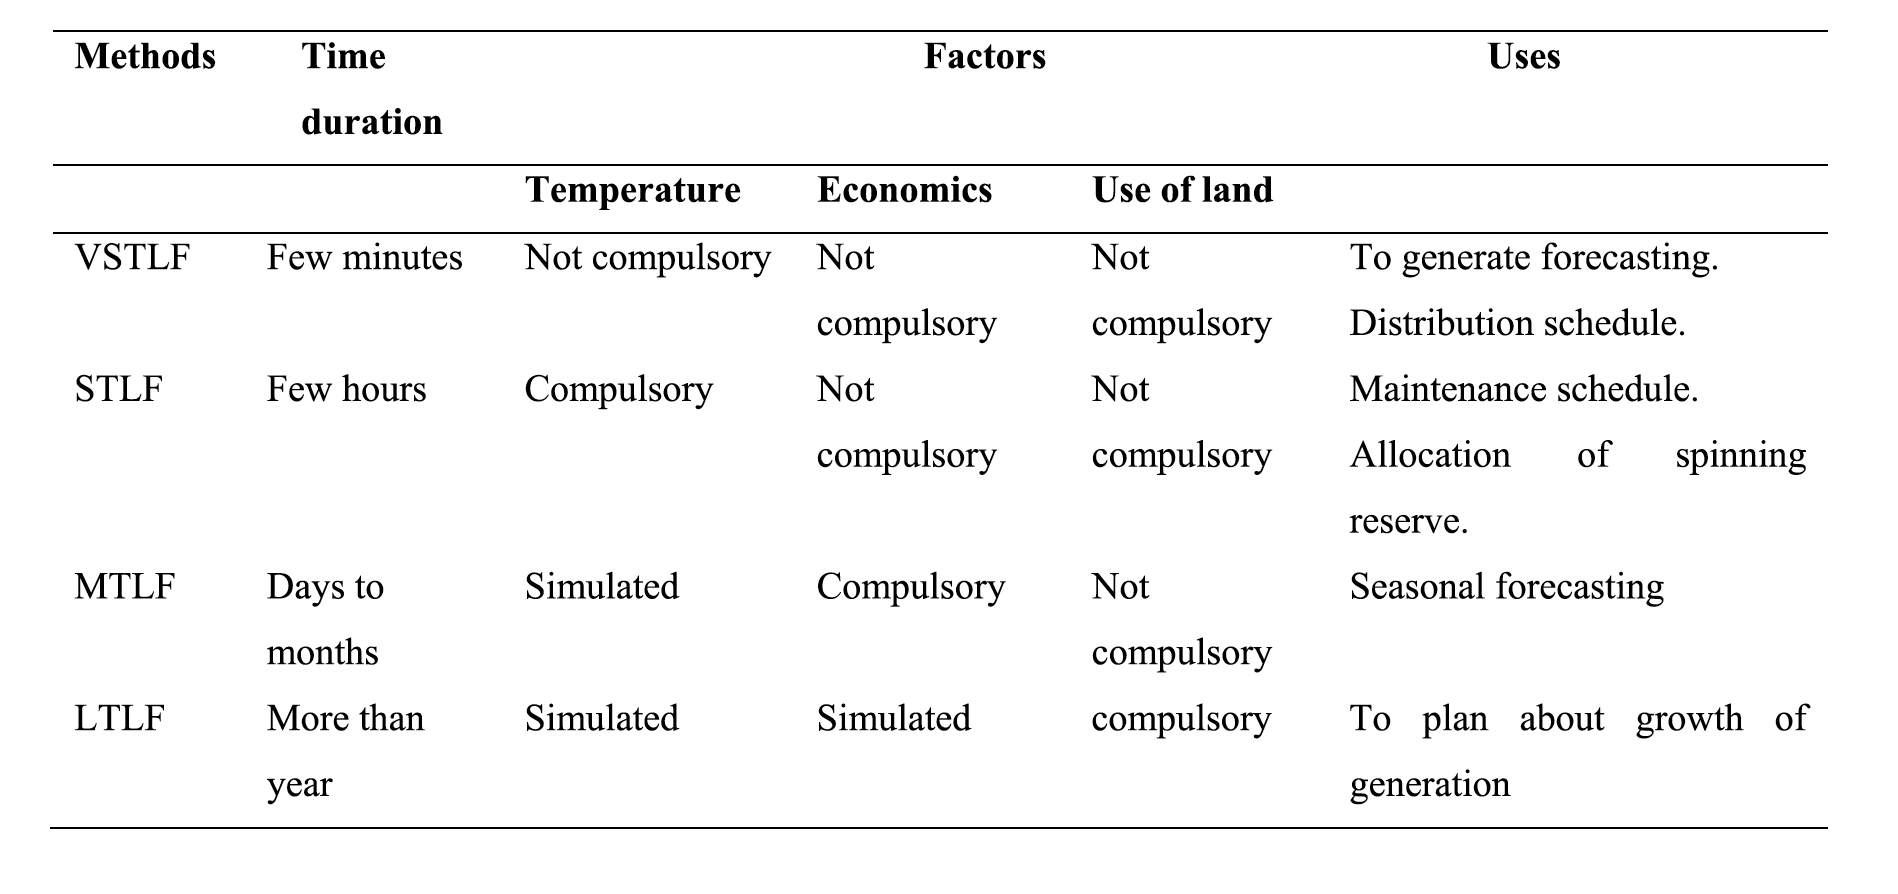
\includegraphics[width=0.95\textwidth, height=5cm]{diff_load_forecasting_methods.png}
\caption{Different load forecasting methods [source: ..]}\label{load_forecasting_methods}
\end{figure}

\section{Forecasting Models}\label{forecasting-models}

Various techniques have been developed for electricity demand
forecasting during the past few years. Statistical models are widely
adopted for the load forecasting problem, which include linear
regression models, stochastic process models, exponential smoothing and
ARIMA models. To incorporate the nonlinearity of electricity demand
series, artificial neural networks (ANNs) have also received substantial
attentions in load forecasting with good performance reported. Neural
networks have been shown to have the ability not only to learn the load
series but also to model an unspecified nonlinear relationship between
load and weather variables. Recently, machine learning techniques and
fuzzy logic approaches have also been used for load forecasting or
classification and achieved relatively good performances.

Techniques such as Artificial Neural Networks (ANNs) and fuzzy logic
models are often used due to their ability to process non-linear
patterns in real-time. For very short-term forecasting, methods that can
capture rapid fluctuations in demand are essential. Additionally,
autoregressive integrated moving average (ARIMA) models and local fuzzy
reconstruction can handle time-series data with high frequency, making
them suitable for forecasting electricity demand in timeframes of
seconds to minutes. These models perform well in scenarios where the
primary objective is operational control, such as maintaining grid
stability or reacting to sudden changes in demand.

For short-term forecasting, covering hours to a few days, models that
integrate external factors such as weather conditions, time of day, and
social behaviour become critical. Generalized Additive Models (GAMs) and
Support Vector Machines (SVMs) are often applied for their ability to
account for non-linear relationships between demand and influencing
variables like temperature, day of the week, and holidays. Hybrid
models, which combine machine learning techniques with statistical
methods like exponential smoothing or seasonal ARIMA, are also effective
for this timeframe, as they can capture both the short-term trends and
seasonal patterns inherent in electricity consumption. \cite{Wang2021}
highlights that although these traditional techniques such as fuzzy
linear regression, exponential smoothing, Automatic Regressive Moving
Average (ARMA) have the advantages of algorithmic simplicity but they
are not scalable to handle large dataset and model complicated
relationships. \textbf{RNNs} are commonly used for load forecasting when
there is a need to model temporal dependencies over shorter sequences.
They are effective in predicting short-term fluctuations in electricity
demand, especially when there is a clear trend or pattern over recent
time intervals, such as hourly or daily demand variations. However,
traditional RNNs suffer from the vanishing gradient problem, which
limits their ability to retain information over long time sequences.
This makes them less effective for capturing long-term dependencies or
seasonal patterns in electricity consumption. To overcome the
limitations of RNNs, \textbf{LSTM networks} are often preferred for load
forecasting, especially when dealing with longer time horizons or when
it's important to capture both short-term and long-term trends in
electricity demand. LSTM networks are designed with a memory cell that
can store information for extended periods, allowing the model to retain
past information over long time sequences. This makes LSTMs particularly
effective for \textbf{short-term to medium-term forecasting}, where
demand patterns depend on both recent trends (such as hourly or daily
fluctuations) and more distant patterns (such as weekly or seasonal
cycles). LSTMs are also highly effective when electricity demand is
influenced by a range of factors, such as weather conditions, time of
day, and past consumption trends.

Medium-term forecasting, which spans weeks to months, focuses on
predicting consumption patterns based on broader trends, such as
seasonal variations, economic cycles, and energy market dynamics.
Time-series models like SARIMA (Seasonal ARIMA) and Exponential
Smoothing State Space (ETS) models are widely used for their ability to
capture seasonal effects and trends. Additionally, machine learning
techniques like Gradient Boosting Machines (GBM) or Random Forests can
be leveraged to include more complex interactions between variables,
such as the effect of emerging technologies like rooftop solar panels.
These models are crucial for tasks such as planning maintenance or
scheduling energy generation resources.

For long-term electricity demand forecasting, \textbf{econometric
models} and \textbf{scenario-based models} are often preferred over
short-term forecasting methods like neural networks. This is because
long-term forecasting, which spans months to years, requires capturing
structural trends, external factors, and macroeconomic indicators that
influence electricity demand over extended periods.

The simplest form of forecasting is Moving Average (MA) which predicts
the future values as the average of n previous values. With a larger
window we can smooth out the noise to find the actual tend but the
forecasts will start to lag as we were to go back further and further to
calculate the average. Exponential Smoothing (ETS) eliminates this
problem by exponentially decrease the weights of the averages over time.
This prioritises more recent values over the older values, however, as
the averaging window size increases the overall trend starts to lag
again. Additionally, most real-world time series are not stationary
i.e., the change in mean or variance over time are not the same at
different observation points. Autoregressive Integrated Moving Average
(ARIMA) \cite{box1970time} extends this idea further by modelling the
dependent relationship between an observation and a set of previously
lagged observations by taking the difference of successive values many
times to make the time series stationary. This is like saying that it
will be hot tomorrow since it has been hot so far this week as the high
air temperature had not varied much. In short, the \(ARIMA(p, q, d)\)
model applies a \(d\)th order differencing on a time series and takes
the last p terms in autoregressive way and the include the last q moving
average terms to generate the forecast over a specified time horizon.
However, the ARIMA model does not consider the repeating patterns within
the time series like temperature increases in the daytime while
decreases in night or hotter summer and colder winter. Seasonal ARIMA
(SARIMA) \cite{box1970time} deals with this challenge by taking the
values of \(p\), \(q\), and \(d\) over a season period m instead of the
immediate past. Auto ARIMA \cite{Hyndman2008} scales this process by
finding the best combination of \(<p, q, d>\) automatic way. Typically,
ARIMA models and its other variants forecast very well but it's hard to
scale for large datasets and often too complex to fine tune without
significant domain expertise. The Theta Forecast
\cite{assimakopoulos2000theta} is another well performed model that uses
a parameter \(\theta\) to smooths the local curvature of a time series.
In the original implementation two theta lines are used and the final
forecast is the average of them. Later, \cite{hyndman2002forecasting}
showed that an ETS with a drift term can perform equally to the original
Theta Forecast and since then adopted to most of its later
implementations. \cite{Wang2021} highlights that although these
traditional techniques such as fuzzy linear regression, exponential
smoothing, Automatic Regressive Moving Average (ARMA) have the
advantages of algorithmic simplicity but they are not scalable to handle
large dataset and model complicated relationships.

Another approach is to first apply Fourier Transformation (FT) to
decompose a stationary time series (i.e., removing trends and
seasonality) from time domain to frequency domain as temporal
frequencies. Once decomposed we can then apply Fast Fourier Transform
(FFT) \cite{shannon1948mathematical} to filter out the noise and only
select the few promising frequencies to perform an Inverse Fast Fourier
Transform (IFFT) to reconstruct the time series and add back the trend
and seasonality. Due to its unique properties FFT is a versatile and
fast generic tool to identify trends and noise filtering in time series
and therefore often used as to establish a baseline forecast. A more
recent and very popular Generalised Additive Model (GAM) for regression
technique is \emph{Prophet} \cite{taylor2017facebook}. It is designed to
optimally handle business forecasting tasks featuring time series
captures at the hourly, daily, or weekly level with ideally at least a
full year of historical data. It can also handle missing data and
outliers, strong seasonality effects occurring daily, weekly, yearly,
holidays and other special one-time events that do not necessarily
follow the seasonality patterns. These unique properties make it very
suitable for both short-term and mid-term electricity forecasting as we
will discuss the \emph{Prophet} model in greater details in following
subsection. Instead of finding a single point forecast from a time
series using statistical methods discussed in the previous subsection,
we can also apply probabilistic methods like probabilistic regression or
other machine learning models. In the simplest form to cast a time
series forecasting as regression we need to first convert the
observations i.e., samples as independent and identically distributed.
We can treat the set of time lags over a fixed length sliding window as
independent feature variables and their succeeding time lag as the
corresponding target variable to convert the time series into a dataset
for interpolation using regression. We can also use rolling and seasonal
rolling time window or Exponentially Weighted Moving Averages (EWMA)
instead of sliding window \cite{Roberts1959}. This kind of
transformation using time lags is called time-delay embedding. Another
approach is to embed time into features so that we can train ML models.
For instance, timestamps associated with time series can be treated as
calendar features i.e., time periodicity like year, month, quarter, day,
hour, minutes, seconds, etc. We can also use the timestamps as
monotonically increasing integers and treat them collectively as time
elapsed feature. tsfeatures (??) and tsfresh (??) are two popular
open-source libraries to extract time series features for ML models. One
straightforward way is to use Linear regression and estimate using least
squares to minimise the Mean Squared Errors (MSE)
\cite{lai2005forecasting}. But multi-collinearity in time series can
lead to unstable and unreliable regression models due to the high
correlation between variables caused by trends, seasonality, or lagged
values. Thus, it's difficult to accurately estimate the coefficients and
interpret the relationships between variables. Regularization techniques
like applying L1 and L2 norms e.g., lasso and ridge regressions can help
address multicollinearity in linear regression by penalising large
coefficients. However, we cannot capture the non-linear relationships
within the independent features using a linear model. For example,
sudden increase in air-conditioning usage after temperature reaches a
certain threshold.

A common way to capture such non-linear relationship is to use a
Decision Tree (DT) \cite{Spiliotis2022} and split branches based on
feature importance such as important time lag moment or seasonal
rolling. But a DT can easily overfit as it often relies on specific
feature importances. We can overcome this by using ensemble learning.
Bagging and Radom Forest are two popular ensemble techniques that use a
set of DTs as weak learners. Furthermore, we can use Gradient Boosted DT
(GBDT) technique for sequential learning and its ability to handle
complex relationships for many time series applications. Popular
boosting implementations like XGBoost \cite{chen2020novel} and Light
Gradient Boosting Machine (LightGBM) \cite{salinas2017deepar} employ
techniques like row and column sampling, and optimised tree growth
algorithms to reduce training time for large time series dataset and
improve prediction accuracy.

Now, we shift our focus into forecasting from time series using
supervised learning models like neural network and deep learning.
Transforming time series data for supervised learning models requires
considerations of temporal dependencies and trends. Encoder-Decoder and
Feed Forward Networks (FNNs) are suitable for fixed-length sequences
while Recurrent Neural Networks (RNNs) and Long Short-Term Memory (LSTM)
networks can better handle variable-length sequences and long-term
dependencies. RNNs address the sequential nature of time series data by
incorporating a recurrent connection allowing information from previous
observations to be passed to subsequent ones \cite{Hochreiter1997Long}.
While RNNs are capable of modelling long-term dependencies they suffer
from the vanishing gradient problem. LSTMs, a variant of RNNs,
introduces gates that selectively control the flow of information,
mitigating the vanishing gradient problem. LSTMs have been successfully
applied to a wide range of time series tasks including forecasting,
anomaly detection, and classification \cite{HochreiterSchmidhuber1997}.
Convolutional Neural Networks (CNNs) originally designed for image
processing but later have been adapted for time series analysis too.
CNNs can effectively capture local patterns and dependencies making them
suitable for time series classification and anomaly detection {[}?{]}.
Lastly, Attention mechanisms and Transformers can capture global
dependencies and the importance of different time steps for complex time
series tasks. Attention mechanisms can model long-range dependencies in
sequence-to-sequence tasks. Attention allows the model to focus on
relevant parts of the input sequence when making predictions {[}?{]}.
Transformers leverage self-attention mechanisms to capture dependencies
between different time steps in the input sequence. Transformers have
been shown to outperform RNNs and LSTMs in many sequence modelling tasks
{[}?{]}.

\section{Challenges to Find the Ideal Electricity Load Forecasting
Method}\label{challenges-to-find-the-ideal-electricity-load-forecasting-method}

In this study we focus on short-term demand forecasting which is an
essential instrument in power system planning, operations, and control.
Many operating decisions are based on load forecasts such as dispatch
scheduling of generating capacity, reliability analysis, and maintenance
planning for the generators. Overestimation of electricity demand will
cause a conservative operation which may lead to overproduction or
excessive energy purchase. For instance, in \cite{AEMO} AEMO uses a
monthly regression model based on five years (60 months) of historical
data. The choice of five years data strikes a balance between ensuring
that the model considers only relatively recent univariate consumption
trends and behaviours while being long enough to capture seasonality and
contain enough multivariate observations to be statistically meaningful.
Univariate models, while simpler, often struggle to capture complex
relationships and seasonal patterns in load data. Multivariate models,
incorporating additional factors like temperature, humidity, and
economic indicators, can improve accuracy but introduce challenges in
data collection, preprocessing, and model complexity, thus require
careful feature engineering. Univariate models use only historical
demand data to make future predictions, while multivariate models
consider other variables such as atmospheric variations and calendars
along with historical demand data in the study of STLF
\cite{asi6060100}. \cite{wang2016review,chen2015electricity} both
highlight the limitations of traditional methods and the growing
interest in advanced hybrid techniques. Therefore, the selection of an
ideal forecasting method depends on factors such as data availability,
computational resources, and the desired level of accuracy, making it a
complex and ongoing research area.

\cite{taylor2009forecasting} develops both univariate and multivariate
models and stated that the univariate models had good prediction
capability. In univariate time series models, the historical electricity
demand data are arranged with correlated past lags to capture the demand
patterns even when the data are limited. \cite{mcculloch2001forecasting}
obtains improved accuracy by including the temperature as a variable,
recognising that weather conditions play a crucial role in forecasting
performance. \cite{Fan2012} proposes a semi-parametric additive models
are proposed to estimate the relationships between demand and the driver
variables. Specifically, the inputs for these models are calendar
variables, lagged actual demand observations and historical and forecast
temperature traces for one or more sites in the target power system. The
proposed methodology has been used to forecast the half-hourly
electricity demand for up to seven days ahead for power systems in the
Australian National Electricity Market (NEM). To achieve more efficient
and accurate load forecasting \cite{Suo} establishes a multi-dimensional
short-term load forecasting model based on XGBoost.The decision forest
composed of many decision trees is the final learning model of XGBoost.
It tries to correct the residual of all the previous weak learners by
adding new weak learners. When these learners are combined for final
prediction the accuracy will be higher than that of a single learner.
The selection of appropriate hyper parameters of XGBoost is directly
related to the performance of the model but there is no universal and
scientific method to determine the hyper parameters. In order to reduce
the randomness and blindness, based on the second search of
multi-dimensional grids, a method of hyper parameters optimisation is
proposed. Each hyper parameters combination is attempted in a grid
traversal manner in turn.

\section{Performance Metrics/ Model
Evaluations}\label{performance-metrics-model-evaluations}

To check the correctness of the methods used for the prediction of real
values of load, different criteria are utilized to evaluate the
techniques of load forecasting. The research of many researchers based
on statistical metrics to optimize the precision of their model, newly
developed statistical metrics such as probabilistic load forecasting
metrics. Due to wide adaptation and extraordinary academic values in
industry, literature on probabilistic forecasting is still in developing
phase. The most important static metrics used by researchers are shown
in table:

\begin{longtable}[]{@{}l@{}}
\toprule\noalign{}
\endhead
\bottomrule\noalign{}
\endlastfoot
\end{longtable}

\chapter{Material and Methods}\label{material-and-methods}

\section{Software}\label{software}

R and Python of course are great software for Data Science. Sometimes,
you might want to use \texttt{bash} utilities such as \texttt{awk} or
\texttt{sed}.

Of course, to ensure reproducibility, you should use something like
\texttt{Git} and RMarkdown (or a Jupyter Notebook). Do \textbf{not} use
Word!

\section{Description of the Data}\label{description-of-the-data}

How are the data stored? What are the sizes of the data files? How many
files? etc.

\section{Pre-processing Steps}\label{pre-processing-steps}

What did you have to do to transform the data so that they become
useable?

\section{Data Cleaning}\label{data-cleaning}

How did you deal with missing data? etc.

\section{Assumptions}\label{assumptions}

What assumptions are you making on the data?

\section{Modelling Methods}\label{modelling-methods}

Based on the literature review we in this study we explore the two
popular model - additive model Prophet by Facebook and another one is
the machine learning model XGBoost for short term demand forecasting.
According to our EDA, the demand has high variability during
peak/off-peak, weekdays, hours of the day and most importantly
temperature change.

TBW

\chapter{Exploratory Data Analysis}\label{exploratory-data-analysis}

This is where you explore your data using histograms, scatterplots,
boxplots, numerical summaries, etc.

\begin{Shaded}
\begin{Highlighting}[]
\ImportTok{import}\NormalTok{ numpy }\ImportTok{as}\NormalTok{ np}
\NormalTok{np.random.seed(}\DecValTok{1}\NormalTok{)}
\NormalTok{np.random.normal(}\FloatTok{0.0}\NormalTok{, }\FloatTok{1.0}\NormalTok{, size}\OperatorTok{=}\DecValTok{10}\NormalTok{)}
\end{Highlighting}
\end{Shaded}

\begin{verbatim}
## array([ 1.62434536, -0.61175641, -0.52817175, -1.07296862,  0.86540763,
##        -2.3015387 ,  1.74481176, -0.7612069 ,  0.3190391 , -0.24937038])
\end{verbatim}

\chapter{Analysis and Results}\label{analysis-and-results}

\section{XGBoost}\label{xgboost}

Having a very simple model is always good so that you can benchmark any
result you would obtain with a more elaborate model.

\bigskip

For example, one can use the linear regression model

\[
Y_i = \beta_0 + \beta_1 x_{1i} + \cdots \beta_p x_{pi} + \epsilon_i, \qquad i=1,\ldots,n.
\] where it is assumed that the \(\epsilon_i\)'s are i.i.d.\(N(0,1)\).

\section{Facebook Prophet}\label{facebook-prophet}

TBW

\chapter{Discussion}\label{discussion}

Put the results you got in the previous chapter in perspective with
respect to the problem studied.

\chapter{Conclusion and Further
Issues}\label{conclusion-and-further-issues}

What are the main conclusions? What are your recommendations for the
``client''? What further analysis could be done in the future?

A figure:

\begin{figure}[H]

\includegraphics{unsw-logo.png}
\caption{A caption}\label{myfigure}
\end{figure}

In the text, see Figure \ref{myfigure}.

\chapter*{References}\label{references}
\addcontentsline{toc}{chapter}{References}

\bibliographystyle{elsarticle-harv} 
\bibliography{references}

\chapter*{Appendix}\label{appendix}
\addcontentsline{toc}{chapter}{Appendix}

\section*{\texorpdfstring{\textbf{Codes}}{Codes}}\label{codes}
\addcontentsline{toc}{section}{\textbf{Codes}}

Add you codes here.

\section*{\texorpdfstring{\textbf{Tables}}{Tables}}\label{tables}
\addcontentsline{toc}{section}{\textbf{Tables}}

If you have tables, you can add them here.

Use \url{https://www.tablesgenerator.com/markdown_tables} to create very
simple markdown tables, otherwise use \LaTeX.

\begin{longtable}[]{@{}lcr@{}}
\toprule\noalign{}
Tables & Are & Cool \\
\midrule\noalign{}
\endhead
\bottomrule\noalign{}
\endlastfoot
col 1 is & left-aligned & \$1200 \\
col 2 is & centered & \$12 \\
col 3 is & right-aligned & \$1 \\
\end{longtable}







\end{document}

